\documentclass{classrep}
\usepackage[utf8]{inputenc}


\studycycle{Informatyka, studia dzienne, inż I st.}
\coursesemester{V}
\coursename{Obliczenia naukowe}
\courseyear{2017/2018}
\courseteacher{dr hab. Paweł Zieliński}
\coursegroup{czwartek TN, 11:15}

\author{
  \studentinfo{Agata Jasionowska}{229726}
}

\title{Laboratorium \ppauza Lista 2}
\begin{document}

\maketitle

\section{Zadanie 1}
	\subsection{Opis problemu}
		Ponowne rozwiązanie zadania 5 z listy 1, jednak z wykorzystaniem nieznacznie zmienionych danych (usunięcie ostatnich cyfr w $x_4$ oraz $x_5$). Ta modyfikacja prezentuje się następująco:
		$$ x_4 = 0.5772156649 ~~~ x_4' = 0.577215664$$
		$$ x_5 = 0.3010299957 ~~~ x_5' = 0.301029995$$
		
		W dalszej części sprawozdania wartości iloczynu skalarnego dla niezmienionych danych oznaczane będą jako $I$, zaś po modyfikacji jako $I'$.
	\subsection{Opis rozwiązania}
		W celu obliczenia iloczynów skalarnych użyto kodu zadania 5 listy 1 na zmodyfikowanych zgodnie z treścią zadania danych.
	\subsection{Wyniki}
		Poniższa tabela prezentuje uzyskane wyniki dla czterech algorytmów obliczających iloczyn skalarny, zestawiając rozwiązania dla $I$ oraz $I'$:
		\begin{table}[!h]
        	\centering
        	\footnotesize
			\sisetup{
				table-number-alignment = right,
				table-figures-integer  = 10,
				table-figures-decimal = 16,
				table-figures-exponent=2
			}
			\begin{tabular}{l|S|S} \toprule
				{podpunkt} & {$I$} & {$I'$} \\ \midrule
				&\multicolumn{2}{c}{\texttt{Float32}} \\ \midrule
				$1$ & -0.4999443 & -0.4999443 \\ 
	 			$2$ & -0.4543457 & -0.4543457 \\
	 			$3$ & -0.5 & -0.5 \\
	 			$4$ & -0.5 & -0.5 \\
	 			\midrule
	 			&\multicolumn{2}{c}{\texttt{Float64}} \\ \midrule
	 			$1$ & -0.4999443 & -0.004296342739891585 \\ 
	 			$2$ & -0.4543457 & -0.004296342998713953 \\
	 			$3$ & -0.5 & -0.004296342842280865 \\
	 			$4$ & -0.5 & -0.004296342842280865 \\ \bottomrule
	 		\end{tabular}
	 		\caption{iloczyn skalarny wektorów.}
			\label{table:1}
		\end{table}	
	\subsection{Wnioski}
		Uzyskane wyniki pokazują, że usunięcie cyfr zgodnie z poleceniem nie wpłynęło na rezultaty dla obliczeń w arytmetyce \texttt{Float32}. Wynika to ze względu na stosunkowo niską precyzję obliczeń w przypadku tej arytmetyki. Potwierdza to analiza zapisu bitowego zmienionych wartości - reprezentacja $x_4$ oraz $x_4'$ wygląda tu identycznie, zaś dla $x_5$ różnica pojawia się dopiero na najmniej znaczącym bicie.
		Zupełnie inna sytuacja ma miejsce w przypadku arytmetyki \texttt{Float64} - rozbieżności są bardzo wyraźnie widoczne. Ostatecznie rezultaty są dalekie od oczekiwanych; spowodowane jest to faktem, iż dane wektory są prawie prostopadłe. W przypadku tego problemu nieznaczne zmiany wpływają na duże błędy końcowe, co potwierdza, że zadanie jest źle uwarunkowane.
\section{Zadanie 2}
	\subsection{Opis problemu}
		W co najmniej dwóch wybranych programach do wizualizacji narysować wykres funkcji $f(x)=e^{x}ln(1+e^{-x})$ oraz policzyć granicę $\lim_{x \to \infty} f(x)$.
		%\[ \lim_{x \to \infty} f(x) \]
		
	\subsection{Opis rozwiązania}
		Wykresy zostały narysowane z użyciem programu \texttt{GNUPlot} oraz pakietu \texttt{Gadfly}, zaś granicę policzono przy pomocy funkcji \texttt{limit} języka Julia (\texttt{SymPy}).
	\subsection{Wyniki}
		Uzyskane wykresy przedstawione są na rysunkach poniżej na Rys. \ref{includegraphics:1} oraz Rys. \ref{includegraphics:2}.
		$$\lim_{x \to \infty} f(x) = 1$$.
		
		\begin{figure} 
  			\includegraphics[scale=0.5, width=\textwidth]{zad2/plotGnu.png}
  			\caption{Wykres funkcji w \texttt{GNUPlot}}
  			\label{includegraphics:1}
  		\end{figure}
  		
  		\begin{figure}
  			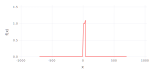
\includegraphics[scale=0.5, width=\textwidth]{zad2/plotGadfly.png}
			\caption{Wykres funkcji w \texttt{Gadfly}}
			\label{includegraphics:2}
		\end{figure}
	\subsection{Wnioski}
		WNIOSKI!!! Obecność fluktuacji: dla Float64 - $x\in (32, 37)$ , Float32 - $x \in (12,20)$
\section{Zadanie 3}
	\subsection{Opis problemu}
		Rozwiązanie układu równań liniowych $Ax = b$ dla danej macierzy współczynników $A \in {\rm I\!R^{n \times n}}$ i wektora prawych stron $b \in {\rm I\!R^n}$ za pomocą algorytmów: eliminacji Gaussa ($x=A/b$) oraz $x = A^{-1}b ~(x=inv(A)*b)$. 
		Macierz $A$ generowana jest w następujący sposób:
		\begin{enumerate}[(a)]
			\item $A = H_n$, gdzie $H_n$ jest macierzą Hilberta stopnia $n$;
			\item $A = R_n$, gdzie $R_n$ jest losową macierzą stopnia $n$ o zadanym wskaźniku uwarunkowania.
		\end{enumerate}
		Przeprowadzenie eksperymentów dla macierzy Hilberta $H_n$ z rosnącym stopniem $n > 1$ oraz dla macierzy losowej $R_n$, $n = 5, 10, 20$ z rosnącym wskaźnikiem uwarunkowania $c = 1, 10, 10^3, 10^7, 10^{12}, 10^{16}$, a także obliczenie błędów względnych.
	\subsection{Opis rozwiązania}
		
	\subsection{Wyniki}
		Hilbert matrix:
		\begin{table}[!h]
        	\centering
        	\footnotesize
			\sisetup{
				table-number-alignment = right,
				table-figures-integer  = 10,
				table-figures-decimal = 16,
				table-figures-exponent=2
			}
			\begin{tabular}{l|S|S|S} \toprule
				{n} & {$|P(z_k)|$} & {$|p(z_k)|$}\\ \midrule
				$1$ & 1.114453504512e13 & 1.3743733197249713e18 \\ 
	 			$2$ & 9.539424609817828e12 & 4.2525024879934694e17 \\
	 			$3$ & 9.539424609817828e12 & 4.2525024879934694e17 \\
	 			$4$ & 3.315103475981763e11 & 2.7420894016764064e16 \\
	 			$5$ & 3.315103475981763e11 & 2.7420894016764064e16 \\ 
	 			$6$ & 1.0612064533081976e11 & 9.545941595183662e14 \\
	 			$7$ & 1.0612064533081976e11 & 9.545941595183662e14 \\
	 			$8$ & 3.357756113171857e10 & 3.2960214141301664e13 \\ 
	 			$9$ & 3.357756113171857e10 & 3.2960214141301664e13 \\
	 			$10$ & 7.143113638035824e9 & 1.4912633816754019e12 \\
	 			$11$ & 7.143113638035824e9 & 1.4912633816754019e12 \\ 
	 			$12$ & 3.065575424e9 & 1.37174317056e11 \\
	 			$13$ & 1.072547328e9 & 1.8525486592e10 \\ 
	 			$14$ & 3.88123136e8 & 1.757670912e9 \\
	 			$15$ & 1.29148416e8 & 2.06120448e8 \\
	 			$16$ & 3.9463936e7 & 4.3303936e7 \\ 
	 			$17$ & 1.046784e7 & 1.0729984e7 \\
	 			$18$ & 2.221568e6 & 2.295296e6 \\ 
	 			$19$ & 349184.0 & 365568.0 \\
	 			$20$ & 20992.0 & 22016.0 \\ \bottomrule
	 		\end{tabular}
	 		\caption{Błędy bezwzględne uzyskanych pierwiastków wielomianu Wilkinsona.}
			\label{table:2}
		\end{table}	
	\subsection{Wnioski}
		WNIOSKI!!!
\section{Zadanie 4}
	\subsection{Opis problemu}
		Przeprowadzenie eksperymentu obliczania zer wielomianu Wilkinsona, zapisanego pod dwiema następującymi postaciami:
		$$P(x) = x^{20}-210x^{19}+20615x^{18} \dots $$
		$$p(x) = (x-20)(x-19)(x-18)\dots (x-2)(x-1)$$
		oraz określenie błędu bezwzględnego wartości tego wielomianu dla otrzymanych pierwiastków.
		Następnie powtórzenie testu dla współczynnika przy $x^{19}$ zmienionego na $-210-2^{-23}$.
	\subsection{Opis rozwiązania}
		Rozwiązanie zadania przygotowano w języku Julia z użyciem trzech funkcji dostępnych w pakiecie \texttt{Polynomials}. Przebiega ono zgodnie z poniższymi krokami:
		\begin{enumerate}[1.]
			\item Utworzenie wielomianu na podstawie podanych współczynników w postaci kanonicznej (funkcja \texttt{Poly}), a także iloczynowej (funkcja \texttt{poly});
			\item Obliczenie pierwiastków wielomianu przy użyciu funkcji \texttt{roots};
			\item Prezentacja błędu bezwzględnego obu postaci wielomianu oraz miejsc zerowych.
		\end{enumerate}
	\subsection{Wyniki}
		\begin{table}[!h]
        	\centering
        	\footnotesize
			\sisetup{
				table-number-alignment = right,
				table-figures-integer  = 10,
				table-figures-decimal = 16,
				table-figures-exponent=2
			}
			\begin{tabular}{l|S|S|S} \toprule
				{k} & {$|P(z_k)|$} & {$|p(z_k)|$}\\ \midrule
				$1$ & 1.114453504512e13 & 1.3743733197249713e18 \\ 
	 			$2$ & 9.539424609817828e12 & 4.2525024879934694e17 \\
	 			$3$ & 9.539424609817828e12 & 4.2525024879934694e17 \\
	 			$4$ & 3.315103475981763e11 & 2.7420894016764064e16 \\
	 			$5$ & 3.315103475981763e11 & 2.7420894016764064e16 \\ 
	 			$6$ & 1.0612064533081976e11 & 9.545941595183662e14 \\
	 			$7$ & 1.0612064533081976e11 & 9.545941595183662e14 \\
	 			$8$ & 3.357756113171857e10 & 3.2960214141301664e13 \\ 
	 			$9$ & 3.357756113171857e10 & 3.2960214141301664e13 \\
	 			$10$ & 7.143113638035824e9 & 1.4912633816754019e12 \\
	 			$11$ & 7.143113638035824e9 & 1.4912633816754019e12 \\ 
	 			$12$ & 3.065575424e9 & 1.37174317056e11 \\
	 			$13$ & 1.072547328e9 & 1.8525486592e10 \\ 
	 			$14$ & 3.88123136e8 & 1.757670912e9 \\
	 			$15$ & 1.29148416e8 & 2.06120448e8 \\
	 			$16$ & 3.9463936e7 & 4.3303936e7 \\ 
	 			$17$ & 1.046784e7 & 1.0729984e7 \\
	 			$18$ & 2.221568e6 & 2.295296e6 \\ 
	 			$19$ & 349184.0 & 365568.0 \\
	 			$20$ & 20992.0 & 22016.0 \\ \bottomrule
	 		\end{tabular}
	 		\caption{Błędy bezwzględne uzyskanych pierwiastków wielomianu Wilkinsona.}
			\label{table:2}
		\end{table}	
		
		
		\begin{table}[!h]
        	\centering
        	\footnotesize
			\sisetup{
				table-number-alignment = right,
				table-figures-integer  = 10,
				table-figures-decimal = 16,
				table-figures-exponent=2
			}
		\begin{tabular}{l|S|S|S} \toprule
				{k} & {$|P(z_k)|$}\\ \midrule
				$1$ & 19.84691021519479 \\ 
	 			$2$ & 17.60966714793733 \\
	 			$3$ & 16.616121458496472 \\
	 			$4$ & 13.037742289370026 \\
	 			$5$ & 12.063218237453977 \\ 
	 			$6$ & 8.379918919523833 \\
	 			$7$ & 7.432242442817582 \\
	 			$8$ & 4.13815012610856 \\ 
	 			$9$ & 3.24599835087197 \\
	 			$10$ & 0.6519586830380406 \\
	 			$11$ & 1.1109180272716561 \\ 
	 			$12$ & 3.0841836320674414 \\
	 			$13$ & 4.992227970900554 \\ 
	 			$14$ & 7.00039792957758 \\
	 			$15$ & 8.999979523326969 \\
	 			$16$ & 11.000001426112089 \\ 
	 			$17$ & 12.999999910275637 \\
	 			$18$ & 15.000000003396579 \\ 
	 			$19$ & 16.99999999994496 \\
	 			$20$ & 19.000000000000163 \\ \bottomrule
	 		\end{tabular}
	 		\caption{Błędy bezwzględne uzyskanych pierwiastków wielomianu Wilkinsona.}
			\label{table:3}
		\end{table}	
		
	\subsection{Wnioski}
		WNIOSKI !!!
\section{Zadanie 5}
	\subsection{Opis problemu}
		Przeprowadzenie dwóch eksperymentów przy wykorzystaniu następującego modelu wzrostu populacji: $$p_{n+1} := p_n + rp_n(1-p_n), \text{ dla } n = 1, 2, \dots,$$
		gdzie $r$ jest pewną stałą, $r(1-p_n)$ jest czynnikiem wzrostu populacji, a $p_0$ jest wielkością populacji stanowiącą procent maksymalnej wielkości populacji dla danego stanu środowiska.
		Testy przeprowadzić dla danych wejściowych we wskazanych arytmetykach:
		\begin{enumerate}[(a)]
			\item $p_0 = 0.01$, $r = 3$, $n = 40$ \{\texttt{Float32}\}
			\item $p_0 = 0.01$, $r = 3$, $n = 40$ \{\texttt{Float64}\}
			\item $p_0 = 0.01$, $r = 3$, $n = 40$, po 10 iteracjach zastosowanie obcięcia wyniku do trzeciego miejsca po przecinku \{\texttt{Float32}\}.
		\end{enumerate}
	\subsection{Opis rozwiązania}
		Rozwiązanie problemu zrealizowano w języku Julia. 
	\subsection{Wyniki}
		Uzyskane rezultaty dla przeprowadzonych eksperymentów:
		\begin{enumerate}[1.]
			\item Zestawienie wyników dla danych (a.) oraz (c.)
				\begin{figure}[h!]
  					\includegraphics[scale=0.5, width=\textwidth]{zad5/plot1.png}
  					\caption{Zestawienie wyników dla danych (a.) oraz (c.).}
				\end{figure}		
			\item Zestawienie wyników dla danych (a.) oraz (b.)
				\begin{figure}[h!] 
  					\includegraphics[scale=0.5, width=\textwidth]{zad5/plot2.png}
  					\caption{Zestawienie wyników dla danych (a.) oraz (b.).}
				\end{figure}
		\end{enumerate}
	\subsection{Wnioski}
		W przypadku pierwszego eksperymentu doskonale można zaobserwować, jak początkowo zdawałoby się znikomy błąd staje się wraz z kolejnymi iteracjami tak duży, iż stanowi oddzielną iterację. !!!
		Analiza drugiego wykresu pozwala dostrzec różnice w regularności przebiegu. Niższa precyzja arytmetyki \texttt{Float32} wpłynęła na stale powiększające się różnice, by osiągnąć swoistą kulminacyjną wartość równą $1.0$. Każda kolejna iteracja oscylowała w pobliżu właśnie tego wyniku.
		Ciekawym spostrzeżeniem jest fakt, iż dla arytmetyki \texttt{Float64} ma miejsce podobna sytuacja, jednak ma ona miejsce w znacznie dalszej iteracji.
		\\ Powyższe eksperymenty pozwalają dostrzec, że błąd obliczeniowy wyniku, przeniesiony jako wejście kolejnej operacji, potęguje powstały błąd. Jest to typowy przykład sprzężenia zwrotnego - procesu, w którym dane wyjściowe jednego problemu są wejściem kolejnych obliczeń.
		W uniknięciu tego rodzaju sytuacji pomóc może zwiększenie precyzji obliczeń, jednak w daleko wybiegających symulacjach powstałe błędy mogą zniekształcić obliczenia w tak dużym stopniu, iż również te wyniki staną się dla badającego bezużyteczne.
\section{Zadanie 6}
	\subsection{Opis problemu}
		Przeprowadzenie eksperymentów w języku \texttt{Julia} w arytmetyce \texttt{Float64} dla następującego równania rekurencyjnego:
		$$x_{n+1} := x^{2}_{n} + c \text{ dla } n = 0, 1, \dots,$$
		gdzie $c$ jest pewną stałą, dla danych wejściowych:
		\begin{enumerate}
			\item $c = -2$ i $x_0 = 1$;
			\item $c = -2$ i $x_0 = 2$;
			\item $c = -2$ i $x_0 = 1.99999999999999$;
			\item $c = -1$ i $x_0 = 1$;
			\item $c = -1$ i $x_0 = -1$;
			\item $c = -1$ i $x_0 = 0.75$;
			\item $c = -1$ i $x_0 = 0.25$;
		\end{enumerate}
		oraz ilości iteracji $n = 40$.
	\subsection{Opis rozwiązania}
		
	\subsection{Wyniki}
%		\begin{figure} 
%  			\includegraphics[scale=0.5, width=\textwidth]{zad6/plot3.png}
%  			\caption{3. $c = -2$ i $x_0 = 1.99999999999999$}
%  		\end{figure}
%  		\begin{figure}
%  			\includegraphics[scale=0.5, width=\textwidth]{zad6/plot6.png}
%  			\caption{6. $c = -1$ i $x_0 = 0.75$}
%  			\includegraphics[scale=0.5, width=\textwidth]{zad6/plot7.png}
%  			\caption{7. $c = -1$ i $x_0 = 0.25$}
%  			W książce "Fraktale granice chaosu" nazywane jest to stabilnością.
%		\end{figure}
	\subsection{Wnioski}
\end{document}
